\documentclass[../main/main.tex]{subfiles}

\newdate{date}{05}{10}{2020}

% \begin{figure}[h!]
% \centering
% \includegraphics[page=6,width=0.8\textwidth]{../lessons/pdf_file/05_lecture.pdf}
% \end{figure}

%\displaydate{date}. Compiled:  \today. Alice.

\begin{document}

\pagestyle{plain}

\section{Lecture 5}


\subsubsection*{Slide 1}

\begin{minipage}[]{0.5\linewidth}
\centering
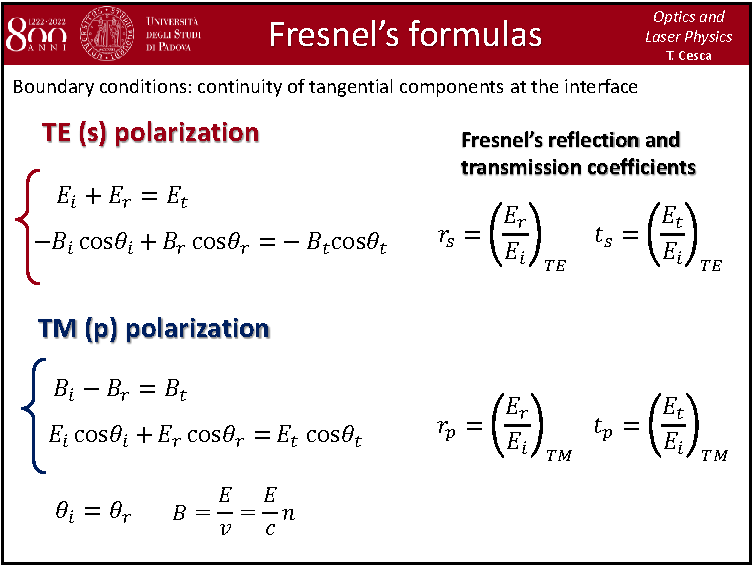
\includegraphics[page=1,width=1\textwidth]{../lessons/pdf_file/05_lecture.pdf}
\end{minipage}
\hspace{0.3cm}\vspace{0.3cm}
\begin{minipage}[c]{0.47\linewidth}

We want to see what happens when TE and TM are impinging in the interface between two media for the amplitude.

Firstly, we have to consider the boundary condition at the interface assuming continuity for the tangential component.

We have also the reflection law and the relation between electric and magnetic field ampltidues.

If we solve this system we can determing the \textbf{Fresnel's reflection and trasmission coefficients}.

\end{minipage}

\subsubsection*{Slide 2}

\begin{minipage}[]{0.5\linewidth}
\centering
\includegraphics[page=2,width=1\textwidth]{../lessons/pdf_file/05_lecture.pdf}
\end{minipage}
\hspace{0.3cm}\vspace{0.3cm}
\begin{minipage}[c]{0.47\linewidth}

You end up with different equations for \textbf{reflection coefficients} and \textbf{transmission coefficients}. All the different ways in which you can write these coefficients is related to the way in which you can write the trigonometric formulas.

\end{minipage}

\subsubsection*{Slide 3}

\begin{minipage}[]{0.5\linewidth}
\centering
\includegraphics[page=3,width=1\textwidth]{../lessons/pdf_file/05_lecture.pdf}
\end{minipage}
\hspace{0.3cm}\vspace{0.3cm}
\begin{minipage}[c]{0.47\linewidth}

The reflections and trasmission coefficients can be rewritten by applying also the Snell's law.

Let us see what are the expressions of the coefficients at normal incidence. The two polarization states are degenerate so we should expect the same cofficients for TE and TM.

The reflection coefficients could be positive or negative according to the value of \( n \). A negative reflection coefficients means that the phase of your reflected wave is 180° wrt the incidence beam.

\end{minipage}

\newpage

\subsubsection*{Slide 4}

\begin{minipage}[]{0.5\linewidth}
\centering
\includegraphics[page=4,width=1\textwidth]{../lessons/pdf_file/05_lecture.pdf}
\end{minipage}
\hspace{0.3cm}\vspace{0.3cm}
\begin{minipage}[c]{0.47\linewidth}

The last thing we note (\( r<1 \)) has interesting consequences. Let us imagine to be able to increase the intensity of a laser beam incident on a glass window. Which side of the window will be damaged earlier?

The answer is the \textbf{backside}, this is because of the phase shift. The phase shift in the front surface is 180° (incidence wave and reflected wave are out of phase). In the back surface they are in phase. If you calculate the intensity of the beam on the back surface, you obtain that it is 44$\%$ higher than for the front side!

\end{minipage}

\subsubsection*{Slide 5}

\begin{minipage}[]{0.5\linewidth}
\centering
\includegraphics[page=5,width=1\textwidth]{../lessons/pdf_file/05_lecture.pdf}
\end{minipage}
\hspace{0.3cm}\vspace{0.3cm}
\begin{minipage}[c]{0.47\linewidth}

\textbf{Reflectance} is the ratio between the power of the reflected beam wrt the power of the incidence beam. Since we are in the same medium the angle of incidence and refraction are the same, the \textbf{footprint} of the incidence beam will be the same of the reflected beam, so you can cancel the area term in the reflectance. So that you obtain \( R = \abs{r}^2  \).

We have to distinguish the reflectance for TE and TM.

At normal incidence, for \( n_1=1 \) and \( n_2 = 1.5 \), we obtain \( R=0.04 \). This means that at the interface between air and common glass the percentage of the incidence power that is reflected is about 4 $\%$. So you will lose 4 $\%$ of the incidence beam.

At grazing incidence, it is easy to calculate that the reflectance is indipendent on \( n \). So, for any medium, if you look close to 90°, will have \( R \) of the order of 1, so it would be highly reflecting.

\end{minipage}

\subsubsection*{Slide 6}

\begin{minipage}[]{0.5\linewidth}
\centering
\includegraphics[page=6,width=1\textwidth]{../lessons/pdf_file/05_lecture.pdf}
\end{minipage}
\hspace{0.3cm}\vspace{0.3cm}
\begin{minipage}[c]{0.47\linewidth}

THe \textbf{Transmittance} coefficient is the power of the transmitted beam divided by the power of  the incidence beam. Since we are passing from media with different refractive index, the footprint (beam diameter) of the beam will be different (they follow the Snell's law).

At normal incidence, for \( n_1 =1 \) and \( n_2 =1.5 \) you will get \( T=0.96 \).

At any angle of incidence we have to satisfy the \textbf{conservation of energy}:
\begin{equation*}
  R + T = 1
\end{equation*}
because we are considering media which are not absorbing.

If we have a stack of optical elements, we have to be aware that we have a portion of the energy that can be reflected that it is not negligible!

\end{minipage}

\newpage

\subsubsection*{Slide 7}

\begin{minipage}[]{0.5\linewidth}
\centering
\includegraphics[page=7,width=1\textwidth]{../lessons/pdf_file/05_lecture.pdf}
\end{minipage}
\hspace{0.3cm}\vspace{0.3cm}
\begin{minipage}[c]{0.47\linewidth}

This happens because at the interface of the window you will get that a portion of the light inside is reflected and trasmitted outside and the same for the light outside. But, in an illuminated room, the internal light reflected by the windows will be much larger than the light trasnmitted from outside. This is why the window look like a mirror at the night.

\end{minipage}

\subsubsection*{Slide 8}

\begin{minipage}[]{0.5\linewidth}
\centering
\includegraphics[page=8,width=1\textwidth]{../lessons/pdf_file/05_lecture.pdf}
\end{minipage}
\hspace{0.3cm}\vspace{0.3cm}
\begin{minipage}[c]{0.47\linewidth}

Let us look at the reflection coefficient \( r \) for the two polarization state as a function of the angle of incidence.

The reflection coefficient for p polarization has a specific angle for which it goes to zero. This is called \textbf{Brewster's angle}: coefficient for which the \( r_p \) goes to zero.

We talk about \textbf{external reflection} when we are passing from a medium with a smaller refractive index toward a medium with a larger one.

The Brewster angle can be observed laso for an \textbf{internal reflacting} (from a larger to a smaller refractive index).

The Brewster's angle is the angle for which the sum with the transmitted angle is equal to \( \pi /2 \).

\end{minipage}

\subsubsection*{Slide 9}

\begin{minipage}[]{0.5\linewidth}
\centering
\includegraphics[page=9,width=1\textwidth]{../lessons/pdf_file/05_lecture.pdf}
\end{minipage}
\hspace{0.3cm}\vspace{0.3cm}
\begin{minipage}[c]{0.47\linewidth}

At Brewster, the refractied ray and the reflected are perpendicular! This happens both for external and internal reflection.

\end{minipage}

\subsubsection*{Slide 10}

\begin{minipage}[]{0.5\linewidth}
\centering
\includegraphics[page=10,width=1\textwidth]{../lessons/pdf_file/05_lecture.pdf}
\end{minipage}
\hspace{0.3cm}\vspace{0.3cm}
\begin{minipage}[c]{0.47\linewidth}


\end{minipage}

\subsubsection*{Slide 11}

\begin{minipage}[]{0.5\linewidth}
\centering
\includegraphics[page=11,width=1\textwidth]{../lessons/pdf_file/05_lecture.pdf}
\end{minipage}
\hspace{0.3cm}\vspace{0.3cm}
\begin{minipage}[c]{0.47\linewidth}

The concept of Brewster's angle is important because if you are impining with TM polarization at \( \theta _B \), the reflection coefficient is 0 (you have no reflection of the beam). This is a way to get negligible reflection.

It is easy to demonstrate that you will get no reflection also at the second interface!

This is widely use in laser media. This is a simple sketch of a laser cavity (solid state laser). The surfaces are cut at Brewster angle. In a laser road the beam will pass thousand of times in order to have amplification. If the reflectance is not null you will use a great amount of energy, so you have to minimize the losses due to reflection. This could be done in two ways: by using low reflectance coatings (but the problems is that they can be damage easily) or place all the optical elements at the Brewster's angle.

\end{minipage}

\subsubsection*{Slide 12}

\begin{minipage}[]{0.5\linewidth}
\centering
\includegraphics[page=12,width=1\textwidth]{../lessons/pdf_file/05_lecture.pdf}
\end{minipage}
\hspace{0.3cm}\vspace{0.3cm}
\begin{minipage}[c]{0.47\linewidth}

This idea can be used also for a polarizer. Let us consider a stack of parallel plate. Let us consider an unpolarized incident beam (superposition of both waves polarized p and s) at Brewster's angle, you have no reflection for p, so the reflected beam will be now polarized s. So, we will have an electric field which is parallel to the interface (or perpendicular to the plane of incidence).

If you use a stack, every time of the reflection, the transmitted beam will be progressively more and more poralized p (\textbf{Stoletov's pile}).

\end{minipage}

\subsubsection*{Slide 13}

\begin{minipage}[]{0.5\linewidth}
\centering
\includegraphics[page=13,width=1\textwidth]{../lessons/pdf_file/05_lecture.pdf}
\end{minipage}
\hspace{0.3cm}\vspace{0.3cm}
\begin{minipage}[c]{0.47\linewidth}

The light come from the rainbow is highly polarized. For the primary arch, the angle of minimum deviation is 138° which correspond to an angle of incidence of 59° and tramitted of 40°. You will see that the Brewster's angle is around 36.9°. This means that the beam is ray is coming in a condition of tramitted angle very close to the Brewster's angle. This means that the p component will not be reflected and the ray that is coming out will be s polarized.

\end{minipage}

\subsubsection*{Slide 14}

\begin{minipage}[]{0.5\linewidth}
\centering
\includegraphics[page=14,width=1\textwidth]{../lessons/pdf_file/05_lecture.pdf}
\end{minipage}
\hspace{0.3cm}\vspace{0.3cm}
\begin{minipage}[c]{0.47\linewidth}

Let us make an exercise.  Whn you are impinging with unpolarized light at a Brewster's angle, the reflected ray is s polarized. So, if you align your linear polarizer in order to minimize the reflected beam, this means that its trasmission axis will be orthogonal to the polarization direction (parallel to the plane of incidence).

\end{minipage}

\subsubsection*{Slide 15}

\begin{minipage}[]{0.5\linewidth}
\centering
\includegraphics[page=15,width=1\textwidth]{../lessons/pdf_file/05_lecture.pdf}
\end{minipage}
\hspace{0.3cm}\vspace{0.3cm}
\begin{minipage}[c]{0.47\linewidth}

We have that
\begin{itemize}
\item \textbf{external reflection}: \( n>1 \)
\item \textbf{internal reflection}: \( n<1 \)
\end{itemize}

In the case of internal reflection, we have again the Brewster's angle but also it is interesting to note that we have a \textbf{critical angle}. The larger is the incidence angle, the more the refracted beam is going far away from the normal at the interface. You will end up in a condition in which the tramitted beam will be parallel to the interface. This is possible only when the relative refractive index is smaller than one.

At angle larger than \( \theta _c \), we are in the \textbf{total internal reflection (TIR) condition}.


\end{minipage}

\subsubsection*{Slide 16}

\begin{minipage}[]{0.5\linewidth}
\centering
\includegraphics[page=16,width=1\textwidth]{../lessons/pdf_file/05_lecture.pdf}
\end{minipage}
\hspace{0.3cm}\vspace{0.3cm}
\begin{minipage}[c]{0.47\linewidth}

The refracted ray will be parallel to the interface.

\end{minipage}

\subsubsection*{Slide 17}

\begin{minipage}[]{0.5\linewidth}
\centering
\includegraphics[page=17,width=1\textwidth]{../lessons/pdf_file/05_lecture.pdf}
\end{minipage}
\hspace{0.3cm}\vspace{0.3cm}
\begin{minipage}[c]{0.47\linewidth}

For angles equal than the critical angle, the modulus of the reflection coefficients is 1 for both \( r_s \) and \( r_s \). But for \( \theta _i > \theta _c \), the coefficients become complex numbers.

\end{minipage}

\subsubsection*{Slide 18}

\begin{minipage}[]{0.5\linewidth}
\centering
\includegraphics[page=18,width=1\textwidth]{../lessons/pdf_file/05_lecture.pdf}
\end{minipage}
\hspace{0.3cm}\vspace{0.3cm}
\begin{minipage}[c]{0.47\linewidth}

This is a nice example of total internal reflection, when you look at the sky from water.

\end{minipage}


\subsubsection*{Slide 19}

\begin{minipage}[]{0.5\linewidth}
\centering
\includegraphics[page=19,width=1\textwidth]{../lessons/pdf_file/05_lecture.pdf}
\end{minipage}
\hspace{0.3cm}\vspace{0.3cm}
\begin{minipage}[c]{0.47\linewidth}

There are several applications of this phenomenum. If you have a glass prism and you cut it at 45° (in the middle) and if you imping perpendicular to the face, when you reach the lateral face you are impinging at an angle larger than the critical one, so the beam will be totally reflected.

This idea is used also for \textbf{Porro's prism} for binocola, for seeing the image not reversed (in the right orientation).

Another situation is in \textbf{optical fibers}.

\end{minipage}


\subsubsection*{Slide 20}

\begin{minipage}[]{0.5\linewidth}
\centering
\includegraphics[page=20,width=1\textwidth]{../lessons/pdf_file/05_lecture.pdf}
\end{minipage}
\hspace{0.3cm}\vspace{0.3cm}
\begin{minipage}[c]{0.47\linewidth}

You can calculate the \textbf{acceptance angle} (maximum angle in which you can enter for obtaining totally internal reflection).

\end{minipage}


\subsubsection*{Slide 21}

\begin{minipage}[]{0.5\linewidth}
\centering
\includegraphics[page=21,width=1\textwidth]{../lessons/pdf_file/05_lecture.pdf}
\end{minipage}
\hspace{0.3cm}\vspace{0.3cm}
\begin{minipage}[c]{0.47\linewidth}

Let us consider a glass prism and another prism of the same material with a gap. If you close completely the gap (you consider a unique block of material), you will not get reflection anymore. You use \textbf{index matching fluid} to frustrate total internal reflaction.

\end{minipage}


\subsubsection*{Slide 22}

\begin{minipage}[]{0.5\linewidth}
\centering
\includegraphics[page=22,width=1\textwidth]{../lessons/pdf_file/05_lecture.pdf}
\end{minipage}
\hspace{0.3cm}\vspace{0.3cm}
\begin{minipage}[c]{0.47\linewidth}

This is what is used to realized readers of fingerprints. Let us consider a glass and a beam coming from inside the glass. If you have a roughness in the material (air inside), when you are in contact you are frustrating total internal reflection, while when you have air you get total internal reflaction.

\end{minipage}


\subsubsection*{Slide 23}

\begin{minipage}[]{0.5\linewidth}
\centering
\includegraphics[page=23,width=1\textwidth]{../lessons/pdf_file/05_lecture.pdf}
\end{minipage}
\hspace{0.3cm}\vspace{0.3cm}
\begin{minipage}[c]{0.47\linewidth}

With this idea we can make sensors of fingerprints. Our skin is a medium with a refractive index close to glass, and is a rough surface. When we put our finger in contact with the sensors, there is a laser light and we can see that there will be position in which we will have total internal reflection (white lines) and frustration (black lines).

\end{minipage}


\subsubsection*{Slide 24}

\begin{minipage}[]{0.5\linewidth}
\centering
\includegraphics[page=24,width=1\textwidth]{../lessons/pdf_file/05_lecture.pdf}
\end{minipage}
\hspace{0.3cm}\vspace{0.3cm}
\begin{minipage}[c]{0.47\linewidth}

We can also apply Jones's notation for TE and TM and create what are colled \textbf{reflection and transmission matrices}.

At grazing incidence the reflection matrix becomes simpler.


\end{minipage}


\subsubsection*{Slide 25}

\begin{minipage}[]{0.5\linewidth}
\centering
\includegraphics[page=25,width=1\textwidth]{../lessons/pdf_file/05_lecture.pdf}
\end{minipage}
\hspace{0.3cm}\vspace{0.3cm}
\begin{minipage}[c]{0.47\linewidth}

The phase shift is related to the angle of incidence and to the relative refractive index.

\end{minipage}


\subsubsection*{Slide 26}

\begin{minipage}[]{0.5\linewidth}
\centering
\includegraphics[page=26,width=1\textwidth]{../lessons/pdf_file/05_lecture.pdf}
\end{minipage}
\hspace{0.3cm}\vspace{0.3cm}
\begin{minipage}[c]{0.47\linewidth}

We can construct a polarizer. We have a romb of glass with refractive index \( 1.5 \) (the environment is air). We imping linearly with a linear polarized beam (same amplitude) at 45°. You will get a phase shift of \( \pi/4 \). If the romb is long enough in order to get another phase shift, the outcoming beam will be dephased wrt the incidence polarization. You get a circularly polarized beam (same amplitude but with a phase shift).


\end{minipage}

\end{document}
